\section{Implementación del software}

La implementación práctica de estos enfoques integrados se evidencia principalmente en los sistemas web empresariales y plataformas de soporte, donde la gestión eficiente de usuarios, roles y solicitudes es prioritaria. En este contexto, los frameworks modernos como Laravel \cite{laravel2023guide} y React \cite{react2023patterns} permiten una interacción fluida entre el backend y el frontend, garantizando una arquitectura modular, segura y escalable.

\subsection{Arquitectura MVC en Laravel-React}

Un ejemplo concreto es el desarrollo de un sistema web de mesa de ayuda o gestión de tickets, en el cual cada módulo —autenticación, registro, seguimiento y reportes— se construye como un componente independiente bajo el patrón MVC \cite{mvc2019analysis}, facilitando su mantenimiento y evolución futura. En Laravel \cite{laravel2022performance}, este patrón se articula mediante controladores que orquestan la comunicación entre modelos y vistas, facilitando la gestión de rutas, autenticaciones y control de acceso. React \cite{react2021scalability}, por su parte, amplía este concepto hacia una interfaz declarativa basada en componentes, donde cada unidad de la vista se comporta como un módulo independiente y reutilizable.

La \cref{fig:estructura_mvc} presenta la arquitectura MVC implementada en el sistema Laravel-React.

\begin{figure}[htbp]
    \centering
    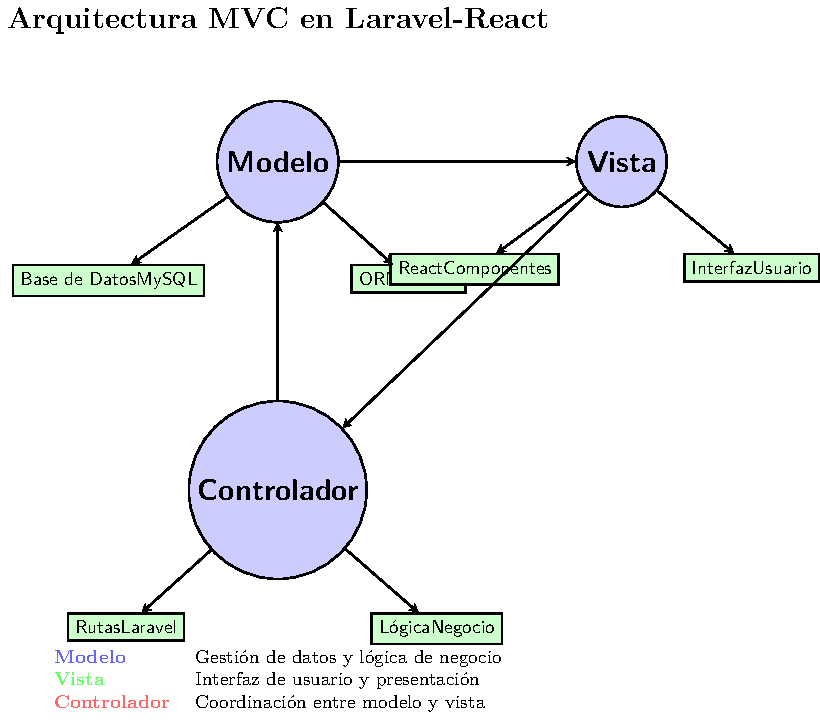
\includegraphics[width=0.8\textwidth]{graphics/estructura_mvc.pdf}
    \caption{Estructura MVC en Laravel–React}
    \label{fig:estructura_mvc}
\end{figure}

\subsection{Gestión de bases de datos}

Los modelos de datos deben diseñarse con criterios de integridad y consistencia. MySQL, combinado con herramientas visuales como PHPMyAdmin, ofrece una base sólida para la creación y gestión de bases de datos relacionales, mientras que la integración con ORM de Laravel facilita la manipulación de datos mediante entidades orientadas a objetos. Este enfoque no solo acelera el desarrollo, sino que permite mantener coherencia entre la capa lógica y la estructura de almacenamiento. Además, el uso de migraciones y seeders en Laravel asegura la trazabilidad y reproducibilidad del entorno de base de datos en diferentes etapas del proyecto.

\subsection{Seguridad informática}

La incorporación de prácticas de seguridad informática es esencial en estos entornos. Desde la definición de la arquitectura hasta la implementación del código, deben considerarse mecanismos de autenticación robustos, encriptación de datos sensibles y control de acceso basado en roles. La tendencia hacia los sistemas cross-platform ha impulsado el desarrollo de esquemas de autenticación unificados, que funcionan tanto en aplicaciones web como móviles. El diseño e implantación de estos sistemas requiere el uso de estándares como OAuth2, JWT y HTTPS, garantizando la protección de la información en todo el ciclo de vida del usuario.

\subsection{Patrón Factory y escalabilidad}

El patrón Factory ha cobrado relevancia al momento de crear objetos de solicitudes, usuarios o servicios, permitiendo una instanciación más controlada y flexible. En sistemas orientados a la escalabilidad, como aquellos basados en Laravel o microservicios, este patrón reduce la dependencia directa del código con las clases concretas, favoreciendo la inyección de dependencias y la facilidad de pruebas unitarias. Combinado con arquitecturas modulares, el patrón Factory permite una organización del sistema por capas y dominios funcionales, lo cual se traduce en mantenibilidad y capacidad de extensión a largo plazo.